%==============================================================================
% Exemplo de Tese de doutorado com a classe texufpel
%
% Adaptação do exemplo de exame de qualificação
% (qualificação/exemplo-qualificacao.tex) para a tese. A pesquisa é a mesma:
% a coleta seletiva de Pelotas com janelas de tempo, agora com os resultados
% finais. O texto de cada seção explica o recurso que aparece nela. As
% diferenças em relação à qualificação estão marcadas com "TESE" nos
% comentários: opção tese, ficha catalográfica, colaborador, banca de quatro
% membros, resultados finais e o fim do cronograma.
% Para começar o seu trabalho, copie este arquivo, troque os dados do
% preâmbulo (os comentários "ALTERE" indicam o que mudar) e substitua o texto
% dos capítulos.
%
% Compilação (a partir da pasta raiz do repositório, onde estão a classe, o
% estilo abnt.bst, o bibliografia.bib e a pasta imagens/):
%   pdflatex tese/exemplo-tese
%   bibtex   exemplo-tese
%   pdflatex tese/exemplo-tese
%   pdflatex tese/exemplo-tese
% No Overleaf, basta marcar tese/exemplo-tese.tex como documento principal.
%
% As páginas citadas nos comentários são as do Manual de normas UFPel para
% trabalhos acadêmicos (2023).
%==============================================================================

% Opções da classe:
%   tese     tese de doutorado (TESE; use tcc, diss, eq, diss-proposta...
%            para os outros tipos)
%   capa     gera a capa (obrigatória no trabalho depositado, Manual, p. 12)
%   english  rótulos em inglês (Abstract, Contents, Figure...), para tese
%            escrita em inglês, se o programa permitir
\documentclass[tese,capa]{texufpel}

%------------------------------------------------------------------------------
% Pacotes usados neste exemplo. Nenhum é obrigatório: carregue só o que o seu
% trabalho usar. A classe já carrega graphicx, hyperref, natbib e caption.
%------------------------------------------------------------------------------
\usepackage{amsmath}        % equações alinhadas (align) e \eqref
\usepackage{algpseudocode}  % pseudocódigo (ambiente algorithmic)
\usepackage{listings}       % listagens de código-fonte
\usepackage{pdfcomment}     % \pdftooltip: dica com o significado da sigla

% Referência completa em nota de rodapé (\footcite). O Manual adota o sistema
% autor-data (p. 62); use este recurso só se o curso pedir.
\usepackage{bibentry}
\nobibliography*
\newcommand{\footcite}[1]{\footnote{\bibentry{#1}}}

% Palavras do pseudocódigo em português
\algrenewcommand\algorithmicrequire{\textbf{Entrada:}}
\algrenewcommand\algorithmicensure{\textbf{Saída:}}
\algrenewcommand\algorithmicfor{\textbf{para}}
\algrenewcommand\algorithmicforall{\textbf{para cada}}
\algrenewcommand\algorithmicdo{\textbf{faça}}
\algrenewcommand\algorithmicwhile{\textbf{enquanto}}
\algrenewcommand\algorithmicif{\textbf{se}}
\algrenewcommand\algorithmicthen{\textbf{então}}
\algrenewcommand\algorithmicend{\textbf{fim}}
\algrenewcommand\algorithmicreturn{\textbf{retorne}}

% Aparência das listagens de código: fonte monoespaçada pequena, linhas
% numeradas e acentos aceitos nos comentários.
\lstset{
  basicstyle=\ttfamily\footnotesize,
  numbers=left, numberstyle=\tiny, numbersep=6pt,
  frame=single, columns=fullflexible, keepspaces=true,
  breaklines=true, showstringspaces=false, tabsize=2,
  literate={á}{{\'a}}1 {é}{{\'e}}1 {í}{{\'i}}1 {ó}{{\'o}}1 {ú}{{\'u}}1
           {â}{{\^a}}1 {ê}{{\^e}}1 {ô}{{\^o}}1 {ã}{{\~a}}1 {õ}{{\~o}}1
           {ç}{{\c{c}}}1 {à}{{\`a}}1 {Á}{{\'A}}1 {É}{{\'E}}1 {Ç}{{\c{C}}}1
}

%------------------------------------------------------------------------------
% Dados institucionais. ALTERE para o seu programa.
% Na pós-graduação, informe o \programa. \curso é a área do título:
% "Doutor em Ciência da Computação".
% Se a unidade for feminina (Faculdade, Escola), use \unidade[a]{...}: a
% folha de rosto passa a dizer "do Programa ... da Faculdade" (Manual, p. 85).
%------------------------------------------------------------------------------
\unidade{Centro de Desenvolvimento Tecnológico}
\programa{Programa de Pós-Graduação em Computação}
\curso{Ciência da Computação}

% Versões em inglês, usadas na referência do abstract
\unidadeeng{Technology Development Center}
\programaeng{Graduate Program in Computing}
\cursoeng{Computer Science}

%------------------------------------------------------------------------------
% Dados do trabalho. ALTERE.
% \author{Sobrenome}{Prenomes}: o sobrenome vai em maiúsculas na referência
% do trabalho, no resumo e no abstract.
% \advisor[título]{Sobrenome}{Prenomes}, e o mesmo para \coadvisor.
%
% Os nomes abaixo são de grandes nomes da Computação e servem só de exemplo.
% Substitua pelos nomes da sua orientação e da sua banca.
%------------------------------------------------------------------------------
\title{Roteamento de veículos com janelas de tempo aplicado à coleta seletiva urbana}

\author{Lovelace}{Ada}                          % ALTERE: autor(a)
\advisor[Prof.ª~Dr.ª]{Liskov}{Barbara}          % ALTERE: orientador(a)
\coadvisor[Prof.~Dr.]{Dijkstra}{Edsger W.}      % ALTERE: coorientador(a), opcional

% TESE: colaborador(a), opcional. Aparece na folha de rosto, abaixo da
% orientação, mas não entra na referência do trabalho. Até quatro, como
% \advisor e \coadvisor.
\collaborator[Prof.~Dr.]{Tarjan}{Robert E.}     % ALTERE ou apague

% \date{mês}{ano} fixa o ano da capa, da folha de rosto e da referência do
% trabalho. Sem este comando, a classe usa o ano em que o documento é
% compilado. ALTERE.
\date{abril}{2030}

% Palavras-chave: iniciais minúsculas (exceto nomes próprios), separadas por
% ponto e vírgula, a última terminada em ponto (Manual, p. 15). Até 10.
\keyword{busca local;}
\keyword{coleta seletiva;}
\keyword{janelas de tempo;}
\keyword{logística urbana;}
\keyword{problema de roteamento de veículos.}

\keywordeng{local search;}
\keywordeng{selective waste collection;}
\keywordeng{time windows;}
\keywordeng{urban logistics;}
\keywordeng{vehicle routing problem.}

\begin{document}

% Orientadora ou coorientadora: troque o rótulo. Com mais de uma pessoa,
% troque também o plural (\advisorsname, \coadvisorsname).
\renewcommand{\advisorname}{Orientadora}
% \renewcommand{\coadvisorname}{Coorientadora}

\maketitle   % capa e folha de rosto

% TESE: a tese é depositada na biblioteca e tem ficha catalográfica. Sem
% argumento, o comando gera uma página provisória. Quando a biblioteca enviar
% a ficha em PDF, use \fichacatalografica[ficha.pdf] (Manual, p. 12).
\fichacatalografica

% Errata (opcional; Manual, p. 13 e 87): vai logo após a folha de rosto e só
% existe se o trabalho já impresso tiver erros a corrigir. Cada linha traz a
% folha, a linha, o texto errado e o texto correto. Descomente para usar.
% \begin{errata}
% 21 & 4 & Dantzig e Ramsey & Dantzig e Ramser \\
% \end{errata}

%------------------------------------------------------------------------------
% Folha de aprovação (Manual, p. 13 e 89). O argumento é a data da defesa.
% TESE: a classe escreve "Tese aprovada, como requisito parcial para
% obtenção do grau de Doutor..."; a banca de doutorado costuma ter mais
% membros que a de mestrado.
% ALTERE os nomes, a titulação e a instituição de cada membro da banca.
%------------------------------------------------------------------------------
\begin{aprovacao}{26 de abril de 2030}
\noindent Prof.ª Dr.ª Barbara Liskov (Orientadora)\\
Doutora em Ciência da Computação pela Stanford University\\[1cm]

\noindent Prof. Dr. Donald E. Knuth\\
Doutor em Matemática pelo California Institute of Technology\\[1cm]

\noindent Prof.ª Dr.ª Grace Hopper\\
Doutora em Matemática pela Yale University\\[1cm]

\noindent Prof. Dr. Leslie Lamport\\
Doutor em Matemática pela Brandeis University
\end{aprovacao}

% Elementos opcionais: dedicatória, agradecimentos e epígrafe
\begin{dedicatoria}
Às equipes de coleta seletiva, que percorrem a cidade todos os dias.
\end{dedicatoria}

% Quem tem bolsa ou outro apoio da CAPES deve incluir a frase
% do último parágrafo, exigida pela Portaria CAPES n.º 206, de 4 de setembro
% de 2018, no idioma do trabalho. Outras agências têm regras próprias.
\begin{agradecimentos}
À professora Barbara Liskov, que acompanhou a pesquisa desde o mestrado e
sugeriu fazer dos horários de coleta o problema central da tese.

Ao professor Edsger W. Dijkstra, pela coorientação, e ao professor Robert E.
Tarjan, que colaborou na formulação exata do problema.

À banca do exame de qualificação, cujas perguntas sobre a solução ótima
mudaram o rumo dos experimentos.

À equipe de coleta do setor 1, que respondeu com paciência a muitas perguntas
sobre horários.

O presente trabalho foi realizado com apoio da Coordenação de Aperfeiçoamento
de Pessoal de Nível Superior -- Brasil (CAPES) -- Código de Financiamento 001.
\end{agradecimentos}

% A epígrafe é uma citação com indicação de autoria (Manual, p. 14). A obra
% citada entra nas referências.
\begin{epigrafe}
I propose to consider the question, ‘Can machines think?’\\
\hspace*{\fill}\citep[p.~433]{Turing:1950:CMI}
\end{epigrafe}

%------------------------------------------------------------------------------
% Resumo: de 150 a 500 palavras, parágrafo único, voz ativa, terceira pessoa
% do singular, sem citações nem siglas (Manual, p. 14). A referência do
% trabalho, acima do texto, é gerada pela classe.
%------------------------------------------------------------------------------
\begin{abstract}
A coleta seletiva em cidades de porte médio costuma seguir rotas definidas
pela experiência das equipes, sem considerar o horário em que cada ponto pode
ser atendido. Esta tese trata a coleta seletiva de Pelotas, no Rio Grande do
Sul, como um problema de roteamento de veículos com janelas de tempo. A malha
viária de quatro setores de coleta foi modelada como um grafo dirigido, para
respeitar o sentido das ruas, e o algoritmo de Dijkstra calculou a matriz de
distâncias entre os pontos. Cada ponto recebeu uma janela de atendimento e um
tempo de serviço, conferidos em campo com a equipe de coleta. Sobre esses
dados, uma heurística de inserção constrói as rotas, e uma busca local as
melhora sem violar as janelas. O problema também foi formulado como programa
linear inteiro, resolvido de forma exata nos dois setores menores para medir
a qualidade da heurística. Nos quatro setores, a busca local reduziu a
distância das rotas em cerca de 3\% em relação à heurística de inserção, com
todos os pontos atendidos dentro da janela. Nos setores em que a solução
exata foi obtida, a heurística ficou a no máximo 1,1\% do ótimo. A tese mostra
que um método simples, montado sobre algoritmos clássicos, produz rotas
viáveis e próximas do ótimo com os dados que a equipe de coleta já possui.
Como limitação, o método supõe um único caminhão por setor e tempos de viagem
fixos, sem variação ao longo do dia.
\end{abstract}

% Abstract: tradução do resumo; o argumento é o título em inglês.
\begin{englishabstract}{Vehicle routing with time windows applied to urban selective waste collection}
Selective waste collection in medium-sized cities usually follows routes set
by the crews' experience, without considering the time at which each point
can be served. This thesis treats selective waste collection in Pelotas, in
the state of Rio Grande do Sul, Brazil, as a vehicle routing problem with
time windows. The road network of four collection sectors was modeled as a
directed graph, to respect the direction of the streets, and Dijkstra's
algorithm computed the distance matrix between points. Each point was given a
service window and a service time, checked in the field with the collection
crew. On these data, an insertion heuristic builds the routes, and a local
search improves them without violating the windows. The problem was also
formulated as an integer linear program, solved exactly in the two smallest
sectors to measure the quality of the heuristic. In all four sectors, local
search reduced route distance by about 3\% relative to the insertion
heuristic, with every point served within its window. In the sectors where
the exact solution was obtained, the heuristic was at most 1.1\% from the
optimum. The thesis shows that a simple method, built on classical
algorithms, yields feasible, near-optimal routes with the data the collection
crew already has. As a limitation, the method assumes a single truck per
sector and fixed travel times that do not vary during the day.
\end{englishabstract}

% Listas: entram depois do abstract e antes do sumário, nesta ordem.
\listoffigures
\listofquadros   % quadros numerados como Figura, em lista própria (Manual, p. 16)
\listoftables

% Lista de abreviaturas e siglas, em ordem alfabética (Manual, p. 18).
% O argumento é a sigla mais longa, para alinhar a coluna dos significados.
% Sigla de expressão estrangeira: significado em itálico.
\begin{listofabbrv}{VRPTW}
  \item[CAPES] Coordenação de Aperfeiçoamento de Pessoal de Nível Superior
  \item[IBGE]  Instituto Brasileiro de Geografia e Estatística
  \item[SBC]   Sociedade Brasileira de Computação
  \item[UFPel] Universidade Federal de Pelotas
  \item[VRPTW] \textit{Vehicle Routing Problem with Time Windows}
\end{listofabbrv}

% Lista de símbolos (Manual, p. 19), na ordem em que aparecem no texto. O
% argumento é o símbolo mais largo, para alinhar os significados.
% Símbolos com colchetes vão entre chaves: \item[{$d[v]$}].
% Os símbolos da Seção 2.5 entram no fim da lista.
\begin{listofsymbols}{$\delta(s, v)$}
  \item[$G$]            grafo
  \item[$V$]            conjunto de vértices
  \item[$E$]            conjunto de arestas
  \item[$w$]            função de peso das arestas
  \item[$p$]            caminho
  \item[$\delta(s, v)$] distância mínima de $s$ até $v$
  \item[{$d[v]$}]       estimativa da distância até $v$
  \item[{$\pi[v]$}]     predecessor de $v$ no caminho mínimo
  \item[{$[a_i, b_i]$}] janela de tempo do cliente $i$
  \item[$s_i$]          tempo de serviço no cliente $i$
  \item[$\tau_{ij}$]    tempo de viagem de $i$ até $j$
  \item[$t_j$]          início do atendimento no cliente $j$
\end{listofsymbols}

\tableofcontents

%==============================================================================
\chapter{Introdução}
\label{cap:introducao}
%==============================================================================

O caminhão da coleta seletiva sai da garagem, passa pelos pontos de coleta e
leva o material até a cooperativa de reciclagem. Em Pelotas, como em muitas
cidades de porte médio, a ordem desses pontos é decidida por quem dirige.
Essa escolha leva em conta o sentido das ruas e o horário de cada ponto: o
comércio do centro põe os resíduos na calçada no fim do expediente, e as
escolas só podem ser atendidas fora do horário de aula. Uma rota mais curta
que chega a um ponto antes de o material estar na calçada obriga o caminhão a
voltar.

O problema de escolher essas rotas é o de roteamento de veículos com janelas
de tempo (\pdftooltip{VRPTW}{Vehicle Routing Problem with Time Windows}, do
inglês \textit{Vehicle Routing Problem with Time Windows}), estudado desde o
trabalho de \citet{Solomon:1987:AVR}. Esta tese aplica esse modelo à coleta
seletiva de Pelotas. O método combina o algoritmo de
\citet{Dijkstra:1959:NTP}, que calcula as distâncias sobre a malha viária,
com uma heurística de inserção e uma busca local, e compara as rotas obtidas
com a solução exata nos setores em que ela pôde ser calculada.

Este documento também é o exemplo de tese da classe \texttt{texufpel},
adaptado do exemplo de exame de qualificação. Cada seção usa um recurso da
classe e explica, no próprio texto, como ele foi feito. Os elementos que
aparecem antes desta página (capa, folha de rosto, ficha catalográfica, folha
de aprovação, dedicatória, agradecimentos, epígrafe, resumo, abstract, listas
e sumário) seguem a ordem do Manual de normas da Universidade Federal de
Pelotas (\pdftooltip{UFPel}{Universidade Federal de Pelotas}) e são gerados
pelos comandos do preâmbulo e pelos ambientes do início do arquivo
\texttt{exemplo-tese.tex}.

Siglas são escritas por extenso na primeira vez em que aparecem, com a sigla
entre parênteses, e entram na lista de abreviaturas e siglas (Manual, p. 18).
Nos parágrafos anteriores, cada sigla foi escrita com o comando
\verb|\pdftooltip|, do pacote \texttt{pdfcomment}, como em
\verb|\pdftooltip{UFPel}{Universidade...}|. O comando mostra o significado
quando o leitor passa o mouse sobre a sigla no PDF. É um recurso de leitura
na tela e não substitui a escrita por extenso na primeira ocorrência.

\section{O que muda em relação à qualificação}

Para transformar o exemplo de qualificação nesta tese, a opção da classe
passou de \texttt{eq} para \texttt{tese}. A classe ajusta sozinha a natureza
do trabalho na folha de rosto (``Tese apresentada ao Programa de
Pós-Graduação em Computação...''), o texto da folha de aprovação, que volta a
trazer ``Data da defesa'', e o tipo de trabalho na referência do resumo,
``Tese (Doutorado em Ciência da Computação)'' (Manual, p. 85, 89 e 94).

Como a tese é depositada na biblioteca, voltam a ficha catalográfica e o
modelo de errata, comentado no arquivo. A folha de rosto ganhou um
colaborador, informado com \verb|\collaborator|, que segue a mesma sintaxe de
\verb|\advisor| e não entra na referência do trabalho. A banca passou a ter
quatro membros, e o ano foi fixado em 2030 com \verb|\date|.

No texto, o capítulo de resultados parciais deu lugar aos resultados finais,
e o capítulo de proposta de continuidade saiu, junto com o cronograma. Se o
programa aceitar teses em inglês, a opção \texttt{english} da classe passa os
rótulos (sumário, listas, legendas) para o inglês.

\section{Objetivos}
\label{sec:objetivos}

O objetivo geral da tese é desenvolver um método de roteamento para a coleta
seletiva que respeite as janelas de tempo dos pontos de coleta e reduza a
distância percorrida. Os objetivos específicos são:

\begin{enumerate}
  \item levantar, com a equipe de coleta, a janela de atendimento e o tempo de
        serviço de cada ponto;
  \item calcular as distâncias entre os pontos com o algoritmo de Dijkstra,
        sobre o grafo dirigido da malha viária;
  \item construir as rotas com uma heurística de inserção, melhorá-las com
        busca local e avaliá-las:
  \begin{enumerate}
    \item pela distância total percorrida;
    \item pela quantidade de pontos atendidos fora da janela;
  \end{enumerate}
  \item comparar a heurística com a solução exata nos setores menores.
\end{enumerate}

A lista acima segue as regras de alíneas do Manual (p. 71): o texto que a
antecede termina em dois pontos, cada alínea começa com letra minúscula e
termina em ponto e vírgula, e a última termina em ponto. A classe formata o
primeiro nível do ambiente \texttt{enumerate} como alíneas, com a), b), c), e o
segundo nível como subalíneas, com travessão. A pontuação fica por conta de
quem escreve.

\section{Organização do texto}

O Capítulo~\ref{cap:fundamentacao} apresenta os conceitos de grafos, o
algoritmo de Dijkstra e o problema de roteamento de veículos e mostra as
formas de citação. O Capítulo~\ref{cap:metodologia} descreve como os dados
foram obtidos e como o método foi construído, com exemplos de figura, quadro
e listagem de código. O Capítulo~\ref{cap:resultados} traz os resultados em
tabela e mostra a numeração das seções até o quinto nível. O
Capítulo~\ref{cap:consideracoes} encerra a tese. Os números dos capítulos
neste parágrafo foram gerados com \verb|\label| e \verb|\ref|: se um capítulo
mudar de lugar, as referências cruzadas se atualizam na próxima compilação.

%==============================================================================
\chapter{Fundamentação teórica}
\label{cap:fundamentacao}
%==============================================================================

\section{Citações}
\label{sec:citacoes}

Este capítulo usa as formas de citação do Manual (p. 62-67). Todas seguem o
sistema autor-data e são feitas com dois comandos do pacote \texttt{natbib}:

\begin{lstlisting}[language={[LaTeX]TeX}, numbers=none]
\cite{Codd:1970:RMD}     % (Codd, 1970)    citação entre parênteses
\citet{Codd:1970:RMD}    % Codd (1970)     autor como parte da frase
\cite[p.~380]{Codd:1970:RMD}   % (Codd, 1970, p. 380)
\end{lstlisting}

A citação indireta reproduz a ideia do autor com outras palavras. O modelo
relacional, por exemplo, propõe que os dados sejam vistos como relações
matemáticas, independentes da forma como estão armazenados
\citep{Codd:1970:RMD}. Quando o autor faz parte da frase, o ano vem entre
parênteses logo depois do nome: \citet{Lamport:1978:TCO} mostrou que, em um
sistema distribuído, a ordem dos eventos pode ser definida sem relógio
global.

Várias obras na mesma citação ficam separadas por ponto e vírgula, de
preferência em ordem alfabética \citep{Hoare:1969:ABC,Lamport:1978:TCO}.
Obras do mesmo autor em anos diferentes aparecem com os anos separados por
vírgula, como em \citet{Turing:1937:OCN,Turing:1950:CMI}. Com quatro ou mais
autores, a citação usa o primeiro seguido de et al. \citep{Cormen:2022:IA}.

A citação direta curta, de até três linhas, fica entre aspas no corpo do
texto, com a página. Para a Sociedade Brasileira de Computação
(\pdftooltip{SBC}{Sociedade Brasileira de Computação}), ``Os cientistas da
computação são responsáveis pela pesquisa e desenvolvimento em Computação''
\citep[p.~30]{Zorzo:2017:RFC}.

A citação direta longa, com mais de três linhas, usa o ambiente
\texttt{quote}. A classe aplica o recuo de 4~cm, a letra tamanho 10 e o espaço
simples que o Manual pede (p. 63). O trecho abaixo foi traduzido de um
documento em inglês, e por isso a chamada termina com ``tradução nossa''
(Manual, p. 66):

\begin{quote}
O protocolo internet é limitado, por definição, às funções necessárias para
entregar um pacote de bits (um datagrama internet) de uma origem a um destino
por meio de um sistema de redes interconectadas. Não há mecanismos para
aumentar a confiabilidade dos dados de ponta a ponta, nem para controle de
fluxo, sequenciamento ou outros serviços comuns em protocolos entre
hospedeiros. O protocolo internet pode tirar proveito dos serviços de suas
redes de suporte para oferecer vários tipos e níveis de serviço
\citep[p.~1, tradução nossa]{Postel:1981:IP}.
\end{quote}

A citação de citação usa a expressão apud. Na lista de referências entra só a
obra consultada (Manual, p. 65). Uma das origens do algoritmo de Bellman-Ford é um
trabalho de 1958 sobre roteamento, que não consultamos diretamente:
\apud{Bellman}{1958}{Cormen:2022:IA} trata do caminho mínimo em grafos que
admitem pesos negativos. Entre parênteses, a mesma citação fica
\apudp{Bellman}{1958}{Cormen:2022:IA}. Os comandos \verb|\apud| e
\verb|\apudp| são da classe; o autor e o ano da obra original são escritos à
mão para que ela não vá para as referências.

Se o curso pedir a referência completa em nota de rodapé, use o comando
\verb|\footcite|, definido no preâmbulo deste arquivo. Ele coloca a referência
no pé da página\footcite{Postel:1981:IP}, e a obra continua na lista de
referências.

\section{Grafos e caminhos mínimos}
\label{sec:grafos}

Um grafo ponderado é um par $G = (V, E)$, em que $V$ é o conjunto de vértices
e $E$ o conjunto de arestas, com uma função de peso $w$ que associa a cada
aresta um número real não negativo \citep{Cormen:2022:IA}. O custo de um
caminho $p = \langle v_0, v_1, \dots, v_k \rangle$ é a soma dos pesos de suas
arestas:
\begin{equation}
  w(p) = \sum_{i=1}^{k} w(v_{i-1}, v_i).
  \label{eq:custo}
\end{equation}

A distância mínima $\delta(s, v)$ entre dois vértices é o menor custo entre
todos os caminhos que os ligam. O algoritmo de Dijkstra mantém uma estimativa
$d[v]$ dessa distância e a melhora por um passo chamado relaxamento, que
testa se passar por $u$ encurta o caminho até $v$:
\begin{align}
  \delta(s, v) &= \min \{\, w(p) : p \text{ é um caminho de } s \text{ até } v \,\},
  \label{eq:delta}\\
  d[v] &\leftarrow \min \{\, d[v],\; d[u] + w(u, v) \,\}.
  \label{eq:relax}
\end{align}

As equações são numeradas com algarismos arábicos entre parênteses, alinhados
à direita (Manual, p. 76). A Equação~\eqref{eq:custo} foi escrita com o
ambiente \texttt{equation}; as Equações~\eqref{eq:delta} e~\eqref{eq:relax},
com \texttt{align}, que alinha as linhas pelo símbolo marcado com \verb|&|.
Para citar uma equação, use \verb|\eqref{rótulo}|.

\section{O algoritmo de Dijkstra}
\label{sec:dijkstra}

O algoritmo resolve o problema do caminho mínimo de origem única quando todos
os pesos são não negativos \citep{Dijkstra:1959:NTP}. A cada passo, ele retira
da fila de prioridade o vértice com a menor estimativa de distância e relaxa
as arestas que saem dele, como mostra a Figura~\ref{fig:dijkstra}.

\begin{figure}[htbp]
  \caption{Pseudocódigo do algoritmo de Dijkstra}
  \label{fig:dijkstra}
  \begin{algorithmic}[1]
    \Require grafo $G = (V, E)$, pesos $w$ não negativos, origem $s$
    \Ensure distâncias $d[v]$ e predecessores $\pi[v]$ para todo $v \in V$
    \ForAll{$v \in V$}
      \State $d[v] \gets \infty$; \quad $\pi[v] \gets \text{nulo}$
    \EndFor
    \State $d[s] \gets 0$
    \State $Q \gets V$ \Comment{fila de prioridade pela chave $d$}
    \While{$Q \neq \emptyset$}
      \State $u \gets$ vértice de $Q$ com menor $d[u]$; remova $u$ de $Q$
      \ForAll{$v$ adjacente a $u$}
        \If{$d[v] > d[u] + w(u, v)$}
          \State $d[v] \gets d[u] + w(u, v)$; \quad $\pi[v] \gets u$
        \EndIf
      \EndFor
    \EndWhile
    \State \Return $d, \pi$
  \end{algorithmic}
  \caption*{Fonte: Adaptado de \citet{Cormen:2022:IA}.}
\end{figure}

O Manual chama de Figura toda ilustração, inclusive esquemas e algoritmos
(p. 16). Por isso o pseudocódigo está dentro de um ambiente \texttt{figure},
com a legenda em cima e a fonte embaixo, e aparece na lista de figuras. O
pseudocódigo foi escrito com o ambiente \texttt{algorithmic}, do pacote
\texttt{algpseudocode}; as palavras-chave em português estão definidas no
preâmbulo deste arquivo.

\section{Outros algoritmos de caminho mínimo}
\label{sec:outros}

Há outros algoritmos para o mesmo problema, cada um com suas restrições. A
Figura~\ref{qua:algoritmos} compara três deles.

\begin{quadro}[htbp]
  \caption{Comparação entre algoritmos de caminho mínimo}
  \label{qua:algoritmos}
  \centering
  \begin{tabular}{|p{2.8cm}|p{2.6cm}|p{4.4cm}|p{4.2cm}|}
    \hline
    \textbf{Algoritmo} & \textbf{Problema} & \textbf{Pesos negativos} & \textbf{Tempo} \\ \hline
    Dijkstra       & origem única       & não aceita & $O((V + E) \log V)$ com heap binário \\ \hline
    Bellman-Ford   & origem única       & aceita e detecta ciclos negativos & $O(VE)$ \\ \hline
    Floyd-Warshall & todos os pares     & aceita, sem ciclos negativos & $\Theta(V^3)$ \\ \hline
  \end{tabular}
  \caption*{Fonte: Elaborado pela autora (2030), com base em \citet{Cormen:2022:IA}.}
\end{quadro}

Um quadro organiza informações textuais e tem as bordas fechadas, ao
contrário da tabela, que apresenta dados numéricos. O Manual não usa o nome
``Quadro'' na legenda: todo quadro é uma Figura, mas pode ter lista própria
quando houver muitos (p. 16). O ambiente \texttt{quadro} da classe faz
exatamente isso: numera junto com as figuras e manda o item para a Lista de
Quadros, gerada por \verb|\listofquadros|.

\section{O problema de roteamento de veículos}
\label{sec:vrp}

O problema de roteamento de veículos foi formulado no fim da década de
1950, para planejar a entrega de combustível a postos a partir de um terminal
\citep{Dantzig:1959:TDP}. Em vez de um caminho entre dois vértices,
procura-se um conjunto de rotas que saem do depósito, atendem todos os
clientes e voltam, com o menor custo total. O problema generaliza o do
caixeiro-viajante e é NP-difícil, classificação que remonta à teoria da
NP-completude iniciada por \citet{Cook:1971:CTP}. Por isso, instâncias reais
costumam ser resolvidas com heurísticas.

Na variante com janelas de tempo, cada cliente $i$ só pode ser atendido
dentro de um intervalo $[a_i, b_i]$ e exige um tempo de serviço $s_i$. Se o
veículo chega antes de $a_i$, espera. Sendo $\tau_{ij}$ o tempo de viagem de
$i$ até $j$, o atendimento em $j$ começa no instante $t_j$ dado pela
Equação~\eqref{eq:inicio}, e a rota só é viável se a
Equação~\eqref{eq:janela} valer para todos os clientes:
\begin{align}
  t_j &= \max \{\, a_j,\; t_i + s_i + \tau_{ij} \,\},
  \label{eq:inicio}\\
  t_j &\le b_j.
  \label{eq:janela}
\end{align}

\citet{Solomon:1987:AVR} propôs heurísticas de construção para essa variante.
A de inserção acrescenta um cliente por vez, na posição de menor custo que
mantém a rota viável. O mesmo trabalho publicou um conjunto de instâncias de
teste que ainda serve de referência na área. Os símbolos desta seção entraram
no fim da lista de símbolos, que segue a ordem em que aparecem no texto
(Manual, p. 19).

\section{Trabalhos relacionados}

Na própria UFPel, \citet{Cruz:2015:FCS} desenvolveu uma ferramenta
computacional para simular a dispersão de poluentes na atmosfera, um exemplo
de como a Computação apoia decisões ambientais da cidade. Esta pesquisa segue
a mesma linha, aplicada à logística da coleta.

%==============================================================================
\chapter{Metodologia}
\label{cap:metodologia}
%==============================================================================

\section{Modelagem da malha viária}

Cada setor de coleta foi modelado como um grafo: os vértices são a
garagem (D), os pontos de coleta (P1 a P4) e a cooperativa de reciclagem (C);
as arestas são os trechos de rua entre eles, com a distância em quilômetros.
Nos trechos de mão única, a aresta tem um só sentido. Cada ponto recebeu,
além disso, uma janela de atendimento e um tempo de serviço, informados pela
equipe de coleta e conferidos em campo entre agosto e outubro de
2028\footnote{Informação fornecida pela equipe de coleta do setor
1 em conversa com a autora, em março de 2028 (informação verbal). Exemplo
fictício de nota de referência para dados não publicados (Manual, p. 69).}. A
Figura~\ref{fig:grafo} mostra o grafo de um dos setores, com a rota mínima de
D até C em destaque.

\begin{figure}[htbp]
  \caption{Grafo de um setor de coleta, com a rota mínima de D até C em destaque}
  \label{fig:grafo}
  \centering
  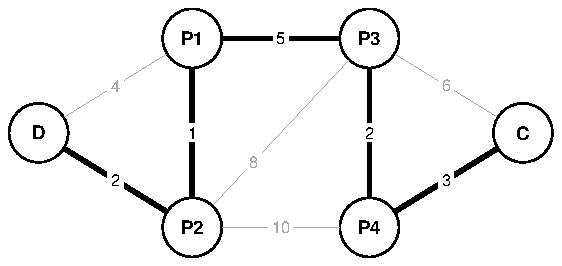
\includegraphics[width=0.75\textwidth]{imagens/grafo-coleta.pdf}
  \caption*{Fonte: Elaborada pela autora (2030).}
\end{figure}

A figura foi inserida com o código abaixo. A legenda vem antes da imagem,
porque o Manual pede a identificação na parte superior, com o número, um
travessão e o título sem ponto final (p. 16). Abaixo da imagem vai a fonte,
obrigatória mesmo quando a figura é da própria autora (p. 17). A classe deixa
a legenda e a fonte em tamanho 10 e espaço simples.

\begin{lstlisting}[language={[LaTeX]TeX}, numbers=none]
\begin{figure}[htbp]
  \caption{Grafo de um setor de coleta, com a rota mínima de D até C em destaque}
  \label{fig:grafo}
  \centering
  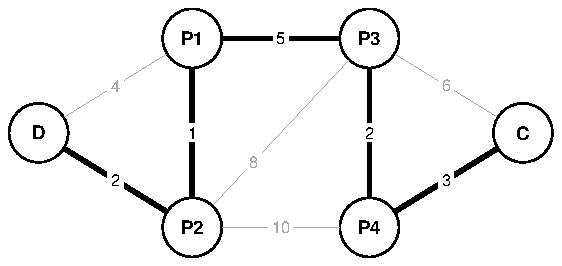
\includegraphics[width=0.75\textwidth]{imagens/grafo-coleta.pdf}
  \caption*{Fonte: Elaborada pela autora (2030).}
\end{figure}
\end{lstlisting}

O caminho da imagem é relativo à pasta onde o documento é compilado, que é a
raiz do repositório. Se a figura vier de outra obra, a fonte traz a citação,
por exemplo \verb|\caption*{Fonte: \citet{Cormen:2022:IA}.}|, e a obra entra nas
referências (Manual, p. 17).

\section{Implementação}

O método tem três etapas, todas escritas em Python. A primeira calcula a
matriz de distâncias: o algoritmo de Dijkstra, com a fila de prioridade do
módulo \texttt{heapq}, é executado a partir de cada ponto. A
Figura~\ref{fig:codigo} mostra a função principal, aplicada ao grafo da
Figura~\ref{fig:grafo}; ao ser executada, ela imprime a distância 13 e o
caminho D, P2, P1, P3, P4, C.

A segunda etapa constrói as rotas com a heurística de inserção de
\citet{Solomon:1987:AVR}. A terceira aplica uma busca local que troca a
posição de dois pontos da rota sempre que a troca reduz a distância e mantém
as Equações~\eqref{eq:inicio} e~\eqref{eq:janela} válidas para todos os
pontos. Para medir a qualidade das rotas, o problema também foi escrito como
programa linear inteiro e resolvido com tempo limite de uma hora por setor.

\begin{figure}[htbp]
  \caption{Implementação do algoritmo de Dijkstra em Python}
  \label{fig:codigo}
\begin{lstlisting}[language=Python]
import heapq

def dijkstra(grafo, origem):
    dist = {v: float("inf") for v in grafo}
    anterior = {v: None for v in grafo}
    dist[origem] = 0
    fila = [(0, origem)]
    while fila:
        d_u, u = heapq.heappop(fila)
        if d_u > dist[u]:
            continue  # entrada antiga da fila
        for v, peso in grafo[u].items():
            if dist[u] + peso < dist[v]:
                dist[v] = dist[u] + peso
                anterior[v] = u
                heapq.heappush(fila, (dist[v], v))
    return dist, anterior

grafo = {
    "D":  {"P1": 4, "P2": 2},
    "P1": {"D": 4, "P2": 1, "P3": 5},
    "P2": {"D": 2, "P1": 1, "P3": 8, "P4": 10},
    "P3": {"P1": 5, "P2": 8, "P4": 2, "C": 6},
    "P4": {"P2": 10, "P3": 2, "C": 3},
    "C":  {"P3": 6, "P4": 3},
}
dist, anterior = dijkstra(grafo, "D")
caminho, v = [], "C"
while v is not None:
    caminho.append(v)
    v = anterior[v]
print(dist["C"], caminho[::-1])  # 13 ['D', 'P2', 'P1', 'P3', 'P4', 'C']
\end{lstlisting}
  \caption*{Fonte: Elaborada pela autora (2030).}
\end{figure}

A listagem foi feita com o ambiente \texttt{lstlisting}, do pacote
\texttt{listings}, dentro de um ambiente \texttt{figure}: assim como o
pseudocódigo, o código-fonte é uma ilustração e recebe o nome de Figura. O
estilo das listagens (fonte, numeração de linhas, moldura e acentos) está no
comando \verb|\lstset| do preâmbulo.

\section{Uso de inteligência artificial}

Na elaboração deste trabalho, utilizou-se a ferramenta de inteligência
artificial generativa [nome e versão da ferramenta], entre [mês/ano] e
[mês/ano], exclusivamente para [finalidades, por exemplo: revisão ortográfica
e tradução do resumo para a língua inglesa]. A ferramenta não foi utilizada
para gerar dados, análises, interpretações ou conclusões. Todo o conteúdo
sugerido foi revisado, editado e validado pela autora, que assume integral
responsabilidade pelo texto final, pela exatidão das informações e pela
autoria intelectual do trabalho.

O parágrafo acima é o modelo de declaração da pasta \texttt{instruções/} do
repositório. Se usar uma ferramenta desse tipo, preencha os trechos entre
colchetes; se não usar, apague a seção.

%==============================================================================
\chapter{Resultados}
\label{cap:resultados}
% TESE: resultados finais, no lugar dos resultados parciais da qualificação.
%==============================================================================

A Tabela~\ref{tab:resultados} mostra a distância das rotas de cada setor
depois de cada etapa do método e, quando o programa linear inteiro terminou
dentro do tempo limite, a distância da rota ótima. Em todas as rotas da
tabela, os pontos foram atendidos dentro da janela.

\begin{table}[htbp]
  \caption{Distância das rotas por setor, em quilômetros}
  \label{tab:resultados}
  \centering
  \begin{tabular}{lrrr}
    \hline
    Setor            & Inserção & Inserção e busca local & Ótimo \\
    \hline
    1 -- Centro      & 16,9 & 16,2 & -- \\
    2 -- Fragata     & 20,6 & 19,9 & 19,9 \\
    3 -- Três Vendas & 23,5 & 22,8 & -- \\
    4 -- Areal       & 18,3 & 17,8 & 17,6 \\
    \hline
    Média            & 19,8 & 19,2 & -- \\
    \hline
  \end{tabular}
  \caption*{Fonte: Elaborada pela autora (2030), com dados fictícios para fins
  de exemplo.}
\end{table}

A busca local reduziu a distância média de 19,8 para 19,2~km, cerca de 3\%.
No setor 2, a rota encontrada é a ótima; no setor 4, ficou 0,2~km acima do
ótimo, uma diferença de 1,1\%. Nos setores 1 e 3, o programa linear inteiro
não terminou em uma hora, e a célula traz um traço.

A tabela segue a padronização do Instituto Brasileiro de Geografia e
Estatística (\pdftooltip{IBGE}{Instituto Brasileiro de Geografia e Estatística}),
indicada pelo Manual (p. 17): traços horizontais no cabeçalho e no fim, sem
traços verticais e sem fechar as laterais. O título vai em cima e a fonte
embaixo, como nas figuras. Valores numéricos ficam alinhados à direita
(\texttt{r} na especificação das colunas). Uma célula sem dado numérico leva
um traço, e o motivo é explicado no texto ou em nota.

\section{Análise por setor}

O setor 1 continua sendo o mais difícil. Tem mais pontos comerciais, com
janelas concentradas no fim da tarde, e é também o maior, o que explica por
que a solução exata não terminou no tempo limite.

\subsection{Setores com traçado regular}

Esta é uma seção terciária. A classe numera as seções até o quinto nível,
como pede o Manual (p. 70), e todas aparecem no sumário em negrito.

\subsubsection{Setor 1 -- Centro}

Esta é uma seção quaternária, criada com \verb|\subsubsection|.

\paragraph{Trecho entre a garagem e o primeiro ponto}

Esta é uma seção quinária, criada com \verb|\paragraph|. Não use níveis abaixo
deste: o Manual limita a numeração progressiva à seção quinária.

%==============================================================================
\chapter{Considerações finais}
\label{cap:consideracoes}
%==============================================================================

A tese partiu de um resultado conhecido: o algoritmo de Dijkstra encurta as
rotas de coleta quando o grafo representa o sentido das ruas. Com as janelas
de tempo, a rota mais curta deixa de ser viável em muitos casos. O método
proposto, que soma a heurística de inserção e a busca local ao cálculo das
distâncias, produziu rotas que respeitam todas as janelas e ficaram próximas
do ótimo nos setores em que ele pôde ser calculado
(Tabela~\ref{tab:resultados}).

O método supõe um único caminhão por setor e tempos de viagem fixos. Tratar
vários caminhões e o trânsito que muda ao longo do dia são os próximos passos
naturais desta pesquisa.

Os apêndices trazem material produzido pela autora: o Apêndice~\ref{apx:dados}
lista os dados do grafo, e o Apêndice~\ref{apx:referencias} mostra como
cadastrar cada tipo de referência. O Anexo~\ref{anx:meses} reproduz material de
outra autoria.

%------------------------------------------------------------------------------
% Referências: estilo abnt.bst e base bibliografia.bib, ambos na raiz.
%------------------------------------------------------------------------------
\bibliographystyle{abnt}
\bibliography{bibliografia}

%------------------------------------------------------------------------------
% Apêndices: material elaborado pela própria autora (Manual, p. 23).
% \apendices cria a folha de abertura; cada \chapter vira "Apêndice A – ...".
%------------------------------------------------------------------------------
\apendices

\chapter{Dados do grafo de exemplo}
\label{apx:dados}

O grafo da Figura~\ref{fig:grafo} tem seis vértices e nove arestas. Os pesos
são as distâncias em quilômetros usadas no código da
Figura~\ref{fig:codigo}: D--P1, 4; D--P2, 2; P1--P2, 1; P1--P3, 5; P2--P3, 8;
P2--P4, 10; P3--P4, 2; P3--C, 6; P4--C, 3. As distâncias mínimas a partir de
D, calculadas pelo algoritmo, são: P2, 2; P1, 3; P3, 8; P4, 10; C, 13.

Apêndices e anexos são numerados com letras e citados no texto pelo nome
seguido da letra, como Apêndice~\ref{apx:referencias} (Manual, p. 23).

\chapter{Exemplos de referências por tipo de documento}
\label{apx:referencias}

Este apêndice cita todas as entradas do arquivo \texttt{bibliografia.bib},
para que a lista de referências deste exemplo mostre como o estilo
\texttt{abnt.bst} formata cada tipo. O arquivo traz, acima de cada entrada, um
comentário explicando quando usar aquele tipo.

Artigos de periódico usam o tipo \texttt{article}:
\citet{Turing:1937:OCN}, \citet{Turing:1950:CMI}, \citet{Shannon:1948:MTC},
\citet{Dijkstra:1959:NTP}, \citet{Dijkstra:1968:GTS}, \citet{Hoare:1969:ABC},
\citet{Codd:1970:RMD}, \citet{Lamport:1978:TCO},
\citet{Dantzig:1959:TDP} e \citet{Solomon:1987:AVR}.

Trabalhos acadêmicos usam \texttt{mastersthesis}, para trabalho de conclusão
de curso e dissertação, como \citet{Cruz:2015:FCS} e \citet{Shannon:1940:SAR},
e \texttt{phdthesis}, para tese, como \citet{Turing:1938:SLO}. Relatórios
técnicos usam \texttt{techreport}: \citet{vonNeumann:1945:FDR} e
\citet{Postel:1981:IP}.

Livros usam \texttt{book}: \citet{vonNeumann:1966:TSR},
\citet{Knuth:1997:ACP}, \citet{Cormen:2022:IA}, \citet{Brooks:1975:MMM},
\citet{Abelson:1996:SIC} e \citet{Moore:1979:MAI}. Um capítulo de livro do
mesmo autor usa \texttt{inbook} \citep{Knuth:1997:IS}; um capítulo de livro
organizado por outra pessoa, \texttt{incollection}
\citep{vonNeumann:1951:GLT}.

Trabalhos publicados em anais de eventos usam \texttt{inproceedings}
\citep{Cook:1971:CTP}; os anais no todo, \texttt{proceedings}
\citep{ACM:1971:STOC}. Normas técnicas usam \texttt{manual}
\citep{ABNT:2018:NBR6023}. Folhetos usam \texttt{booklet}
\citep{Zorzo:2017:RFC}, e documentos não publicados, \texttt{unpublished}
\citep{Dijkstra:1988:CRT}.

Os demais documentos usam \texttt{misc}: preprint
\citep{Vaswani:2017:AIA}, página da web \citep{ACM:2026:TA}, programa de
computador \citep{Aguiar:2026:TEX}, legislação \citep{Brasil:2015:LBI} e
conjunto de dados \citep{Fisher:1936:IRI}.

%------------------------------------------------------------------------------
% Anexos: material de outra autoria (Manual, p. 23-24).
%------------------------------------------------------------------------------
\anexos

\chapter{Abreviatura dos meses em português}
\label{anx:meses}

\begin{table}[htbp]
  \caption{Abreviatura dos meses em português}
  \centering
  \begin{tabular}{llll}
    \hline
    Mês & Abreviatura & Mês & Abreviatura \\
    \hline
    janeiro   & jan.  & julho    & jul. \\
    fevereiro & fev.  & agosto   & ago. \\
    março     & mar.  & setembro & set. \\
    abril     & abr.  & outubro  & out. \\
    maio      & maio  & novembro & nov. \\
    junho     & jun.  & dezembro & dez. \\
    \hline
  \end{tabular}
  \caption*{Fonte: \citet{ABNT:2018:NBR6023}.}
\end{table}

\end{document}
